%=====================
% Remove this after writing actual report
%=====================
%
%Maecenas sed ultricies felis. Sed imperdiet dictum arcu a egestas. 
%\begin{itemize}
%	\item Donec dolor arcu, rutrum id molestie in, viverra sed diam
%	\item Curabitur feugiat
%	\item turpis sed auctor facilisis
%	\item arcu eros accumsan lorem, at posuere mi diam sit amet tortor
%	\item Fusce fermentum, mi sit amet euismod rutrum
%	\item sem lorem molestie diam, iaculis aliquet sapien tortor non nisi
%	\item Pellentesque bibendum pretium aliquet
%\end{itemize}
%\blindtext
%
%Text requiring further explanation\footnote{Example footnote}.

%=====================
%  MATHEMATICS
%=====================
To accomplish our task, we implement a Support-Vector Machine. This method is used to separate data into two different classes by a hyperplane\footnote{A pivotal assumption in our application is that our data (the images of different digits) are indeed linearly separable. We will find that this is mostly true, but not 100\% so.}:
\begin{equation}
\vec{w}\cdot\vec{x} + b = 0
\end{equation}
The two sets' vectors with the minimum distance to each other are defined as the support vectors, and assigned a $y_{i}$ shift of $1$ or $-1$ from the separating hyperplane. These vectors form the two constraints on our optimal hyperplane:
\begin{equation}
\begin{gathered}
	\vec{w}\cdot\vec{x_0} + b \geq 1 \text{ , if } \vec{y_i} = 1 \\
	\vec{w}\cdot\vec{x_1} + b \leq -1 \text{ , if } \vec{y_i} = -1 
\end{gathered}
\end{equation}

Figure \ref{fig:SVM_fig} shows this concept using a Matlab plot

\begin{figure*}[!htb]
	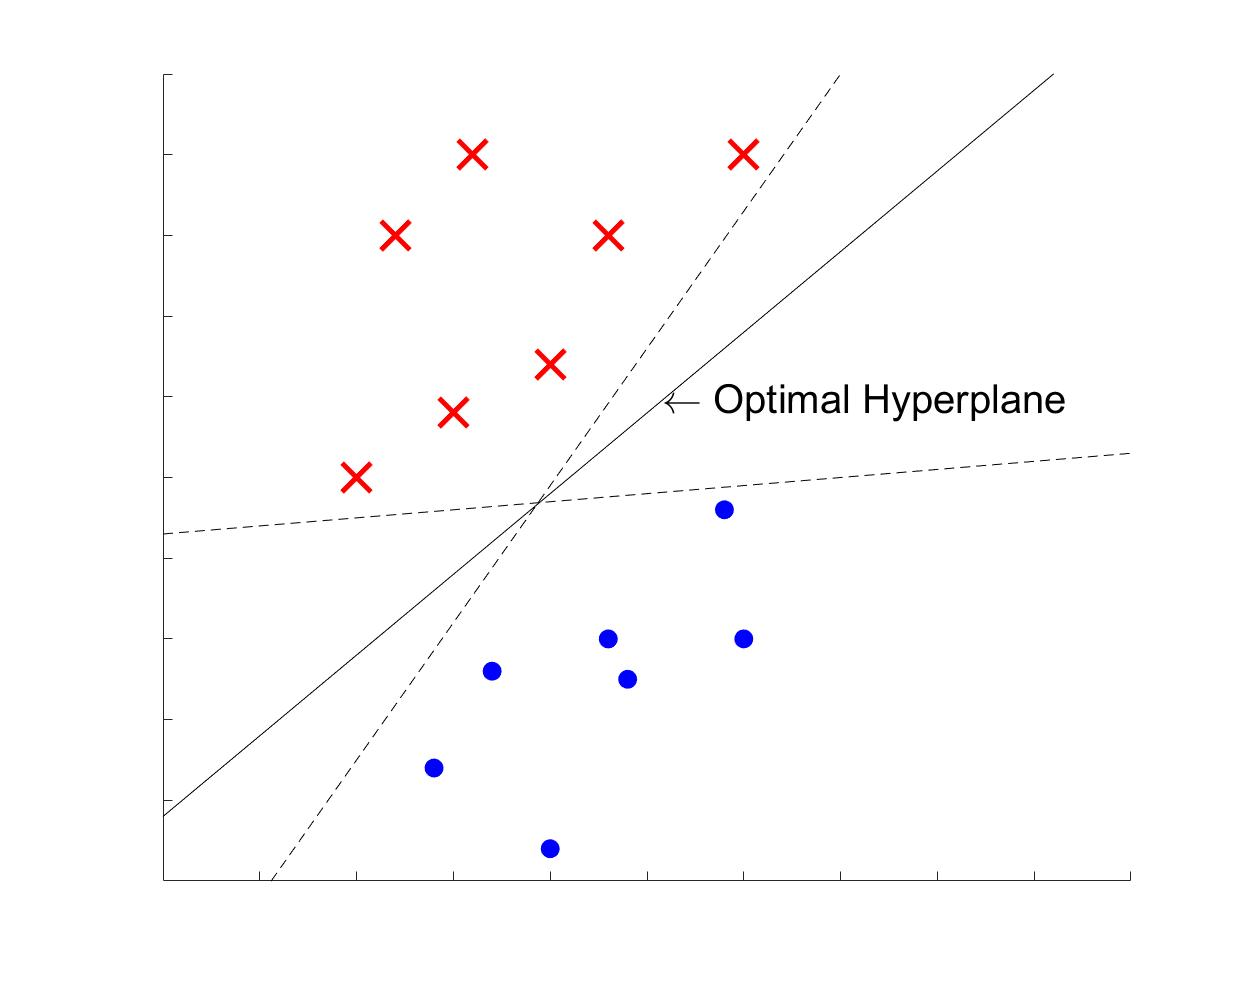
\includegraphics[width=10cm, height=10cm]{SVM_fig}
	\centering
	\caption{The hyperplane is constrained to be within the limits of the margin, which are themselves defined by the support vectors. \cite{matlab}}
	\label{fig:SVM_fig}
\end{figure*}

This form is called canonical, as we have chosen to define $y \in \{-1, 1\}$. The choices of -1 and 1 are arbitrary, but result in the simplest most efficient calculation in computer applications. The set of $y$ values represents our two classes, and must always only have two elements. The problem of applying this to problems with more than 2 cases is discussed later, since our problem is to differentiate between 10 classes of numerical digits.

Furthermore, this application represents the two classes as Class 1 and Not Class 1. Therefore the two classes in this case must be orthogonal compliments to each other in the superspace they both reside. That is: the sum of the dimension of Class 1 and 2 must equal the superspace which they occupy. As an example on the superspace $V = \Re^3$, assume Class 1 is defined by the span of column vectors: 
\begin{equation}
V_{C_{1}} = 
span(\begin{pmatrix}
1 & 0 \\0 & 1\\1& 0
\end{pmatrix}),
\end{equation}

then Class two must be defined as:
\begin{equation}
V_{C_{2}} = span(\begin{pmatrix}
-1\\0\\1
\end{pmatrix}
)
\end{equation}

This is a trivial example, but he beauty of SVMs is that we can define these classes however we like -- as long as we can convert some set of objects into vectors.
\subparagraph{The Optimal Hyperplane}

The optimal hyperplane is defined as the plane that results in zero error and that maximizes the distance from the support vectors. In our use of two canonical classes, this distance can be derived to be $\frac{1}{2}\vec{w}\cdot\vec{w}$, or $\frac{||\vec{w}||}{2}$, and this is shown in the Appendix.

This will maximize the margin of error of the separating plane and thus be the most accurate in determining which class any given input vector belongs to given our dataset. 

The accuracy of the SVM very much depends on the data. If the data is linearly separable, the SVM will be more accurate than a set that is not. With that said, a non-linearly separable dataset can be transformed into a linear dataset using what is called a kernel function. These functions are inherently nonlinear since if we were to have a linear transformation and tried to find a better hyperplane:
\begin{equation}
\begin{gathered}
	L[\vec{x}] = A\vec{x} \\
	\vec{w}\cdot \vec{x} \Rightarrow \vec{w} \cdot \vec{x}^{'} 
\end{gathered}
\end{equation}

